\section{Shear-stress distribution}
The skin friction coefficient $c_f$ distribution is shown in
~\Cref{fig:cf}. It should be noted that the sign of the skin friction
effectively depends on the angle of the tangent vector, for which there
are two possibilities: the tangent vector can either point towards
the leading or trailing edge.

In this case, the tangent direction was chosen using the direction of the flow. This
is relevant to do because it means that regions of negative skin friction coefficient
directly correspond to locations of recirculation since $c_f$ is proportional to
$\partial u/\partial y$.

Thus, for the most part, the tangent was oriented towards the trailing edge.
The only exception to this is the lower surface close the leading edge,
where the flow is actually going towards the leading edge due to the angle of
attack. This is illustrated in~\Cref{fig:stag}. It should also be noted that
$c_f = 0$ at the stagnation point because $\partial u/\partial y = 0$, which explains the
curve corresponding to the lower surface.

Now, several observations can be made using~\Cref{fig:cf}, all of which will
be discussed in detail in~\Cref{sec:bl}.
\begin{enumerate}
    \item The skin friction on the upper surface is significantly higher than on
        the lower surface for the majority of the airfoil length.
    \item On the upper surface, $c_f$ quickly drops down to below zero and shoots back up,
        after which it slowly decreases. This is clearly a case of separated flow which
        reattaches once flow enters the turbulent regime.
    \item On both surfaces, $c_f$ turns negative near the trailing edge. Thus, one can also
        expect a recirculation zone in those regions.
\end{enumerate}

\begin{figure}[H]
    \centering
    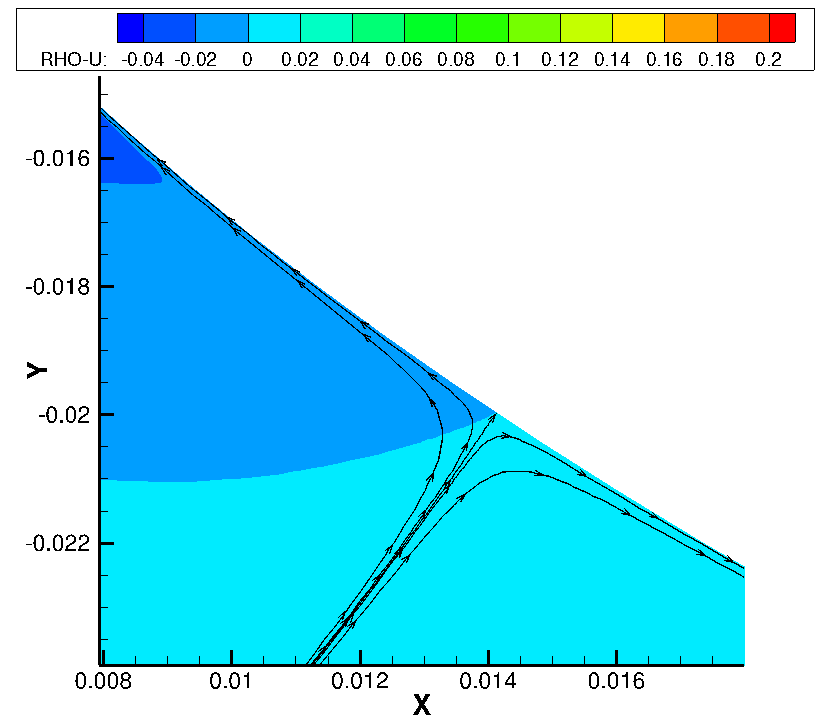
\includegraphics[width=0.5\textwidth]{./figs/stagnation.png}
    \caption{Location of stagnation point can be found on the lower airfoil surface
        just after the leading edge. The flow is going in opposite directions
        on either side of that point.}\label{fig:stag}
\end{figure}

\begin{figure}
    \centering
    \includegraphics[width=\textwidth]{./figs/cf.pdf}
    \caption{Skin friction coefficient over the airfoil surface.}\label{fig:cf}
\end{figure}


